\subsection{Rapid Growth Requires \textit{E. coli} to Increase Both Cell Size and Ribosomal
Mass Fraction}
In \FIG{ribosome_limit}(C) we find that above about 0.75 hr$^{-1}$, the growth
rate is determined by the ribosomal mass fraction $\Phi_R$, since $f_a$ is close
to 1, and $r_t$ is near its maximal rate [cite and refer to figure/
supplemental]. While $\Phi_R$ will need to increase in order for cells to grow faster, the
fractional dependence in \EQ{translation_limit_growth_rate} gives little insight
into how this is actually achieved in the cell and we consider this further here.

It is now well-documented that \textit{E. coli} cells add a constant volume per
origin of replication, which is robust to a remarkable array of cellular
perturbations \citep{si2017}. We find that ribsomal copy number also scales its
ribosome copy number in proportion to $\langle$\# ori$\rangle$
\FIG{translation_ecoli_partA}(A). Importantly, however, it will only be due to
an increase in $\Phi_R$ at these moderate to fast growth rates that cells can
achieve an increase in their growth rate. Indeed, we find that the deviations in
protein expression with $\langle$\# ori$\rangle$ are largely restricted to
regions of ribosomal protein genes \FIG{translation_ecoli_partA}(B). Here we
have calculated the position-dependent protein expression across the chromosome
by a running Gaussian average of protein copy number (20 kbp st. dev. averaging
window) based on each gene's transcriptional start site. These were
median-subtracted to account for the change in total protein abundance with
$\langle$\# ori$\rangle$. This result suggests that $\Phi_R$ is also being tuned
in proportion to $\langle$\# ori$\rangle$ under nutrient-limited growth, and in
particular, it is through this additional dependence on $\Phi_R$ that \textit{E.
coli} exhibits an exponential increase in cell size with growth rate.

% To understand how this relates to growth rate, we
% neeed to consider the changes in proteome composition and ribosome abundance
% with $\langle$\# ori$\rangle$. In \FIG{translation_ecoli_partA}(D),


% For a
% constant cell cycle time $\tau_{cyc}$, which is observed at growth rates above
% about 0.5 hr$^{-1}$ (\FIG{translation_ecoli_partA}(A), \citep{helmstetter1968}),
% \EQ{Nori} states that $\langle \text{\# ori} \rangle$ will need to increase
% exponentially with the growth rate.

%
%
%
% While this says nothing of the observed scaling between cell
% size and growth rate, the additional dependency on ribosomal fraction through
% \EQ{translation_limit_growth_rate} provides an important link.
%
%



%
% To better explore how cells vary protein abundance proteome-wide
% across growth conditions, in \FIG{translation_ecoli_partA}(D), we show that the major deviations
% in protein expression across the chromosome in different growth conditions is a change
% in ribosomal expression.
%
% determined the position-dependent protein expression across the chromosome by
% calculating a running Gaussian average of protein copy number (20 kbp st. dev.
% averaging window) based on each gene's transcriptional start site. These were
% median-subtracted to account for the differences in total protein abundance.
%

%
%
% \subsection{Rapid Growth Requires an Increase in Ribosomal Copy Number and Cell Size}
% In \FIG{ribosome_limit}(C) we find that above about 0.75 hr$^{-1}$, the growth
% rate is dictated by the ribosomal mass fraction $\Phi_R$, since $f_a$ is close
% to 1, and $r_t$ is near its maximal rate [cite and refer to figure/
% supplemental]. While the preceeding section helps us understand that cells will
% need to increase $\Phi_R$ in order to grow faster, the fractional dependence
% gives little insight into how this is actually achieved within the cell. Here we
% consider how the observed changes in absolute protein content
% relate to this dependence between growth rate and $\Phi_R$.
%
% It is now well-documented that \textit{E. coli} cells add a constant volume per
% origin of replication, which is robust to a remarkable array of cellular
% perturbations \citep{si2017}.  The average number of origins per cell, $\langle$\#
% ori$\rangle$, is set by how often replication must be initiated per cell doubling
% under steady state growth. This can be quantified as
% \begin{equation}
%     \langle \text{\# ori} \rangle = 2^{\tau_{cyc} / \tau} = 2^{\tau_{cyc} \lambda / ln(2)},
%     \label{eq:Nori}
% \end{equation}
% where $t_{cyc}$ is the cell cycle time (referring to the time from replication
% initiation to cell division), and $\tau$ is the cell doubling time. To consider
% this  in the context of the proteomic data, we used measurements of $\tau_{cyc}$
% and  $\tau$ from \cite{si2017} (\FIG{translation_ecoli_partA}(A)) to
% calculate $\langle$\# ori$\rangle$  with \EQ{Nori} at different growth
% rates. For ribosomal synthesis, we find an approximately linear correlation
% between ribosome copy number and $\langle$\# ori$\rangle$
% (\FIG{translation_ecoli_partA}(B)).
%
% For a constant cell cycle time, which is observed at growth rates above about
% 0.5 hr$^{-1}$ (\FIG{translation_ecoli_partA}(A), \citep{helmstetter1968}),
% \EQ{Nori} states that $\langle \text{\# ori} \rangle$ will need to increase
% exponentially with the growth rate. While this says nothing of the observed
% scaling between cell size and growth rate, the additional dependency on
% ribosomal fraction through \EQ{translation_limit_growth_rate} provides an
% important link. To better explore how cells vary protein abundance proteome-wide
% across growth conditions, in \FIG{translation_ecoli_partA}(D), we
% determined the position-dependent protein expression across the chromosome by
% calculating a running Gaussian average of protein copy number (20 kbp st. dev.
% averaging window) based on each gene's transcriptional start site. These were
% median-subtracted to account for the differences in total protein abundance.
% Importantly, the major deviations in protein copy number are largely restricted to
% regions of ribosomal protein genes. This suggests that the ribosomal fraction
% $\Phi_R$ is also being tuned in proportion to $\langle$\# ori$\rangle$, and that
% it is through this dependence that \textit{E. coli} exhibits an exponential
% increase in cell volume with growth rate.




\begin{figure*}
    \begin{fullwidth}
    \centering{
        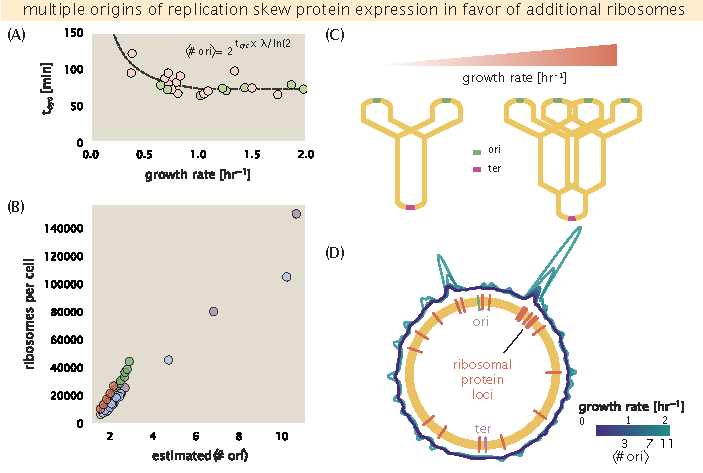
\includegraphics{main_figs/fig8_ribosome_growth_limit_ecoli_a_polar_coord.pdf}
        \caption{\textbf{Cells increase both absolute ribosome abundance and $\Phi_R$ with
        $\langle$\# ori$\rangle$.} (A) Plot of the ribosome copy number estimated from the
        proteomic data against the estimated $\langle$\# ori$\rangle$ (see Appendix
        \nameref{sec:SI_ori} for additional details). (B) A running
        Gaussian average (20 kbp st. dev.) of protein copy number is calculated
        for each growth condition considered by \citep{schmidt2016} based
        on each gene's transcriptional start site. Since total
        protein abundance increases with growth rate, protein copy numbers are
        median-subtracted to allow comparison between growth conditions.
        $\langle$\# ori$\rangle$ are estimated using the data in (A) and
        Equation \ref{eq:Nori}. } \label{fig:translation_ecoli_partA}
    }
    \end{fullwidth}
\end{figure*}
